\documentclass[]{beamer}
\usepackage[T1]{fontenc}
\usepackage[utf8]{inputenc}
\usepackage[english]{babel}
\usepackage[babel]{csquotes}
% Graphics related packages:
\usepackage{tikz,pgfplots,graphicx,siunitx}
\DeclareSIUnit\torr{torr}
\usepackage[mode=buildnew]{standalone}
\usepackage{tikzscale}
\usepackage{ifthen} % used in fiber.tikz
\usetikzlibrary{calc} % used in fiber.tikz
\usetikzlibrary{math} % used in starkBroadening.tikz

%% To reduce compilation time
%\usepgfplotslibrary{external}
%\tikzexternalize

\usepackage{adjustbox} % for \adjincludegraphics for begin{columns}
%Information to be included in the title page:
% For tables:
\title{Low jitter plasma channel in 3D printed gas filled capillary discharges}
\subtitle{Thesis Presentation}
\author{Ehud Behar}
\institute{Hebrew University of Jerusalem}
\date{2021}

\AtBeginSection[]
{
  \begin{frame}
    \frametitle{Table of Contents}
    \tableofcontents[currentsection]
  \end{frame}
} % put the table of contents at the beginning of each section and highlight the title of the current section

% from https://tex.stackexchange.com/a/415653/180429
\setbeamertemplate{frametitle continuation}{\insertcontinuationcount}
\begin{document}

\frame{\titlepage}
\begin{frame}
\frametitle{Table of Contents}
\tableofcontents
\end{frame}

\section{Background}
\subsection{Theoretical Introduction}
  \begin{frame}{Linear accelerators}
  \begin{center}
    The goal --- design a table--top particle accelerator.
  \end{center}
    Applications:
    \begin{itemize}
        \item[\textbullet] Experiments on the structure of matter
        \item[\textbullet] Creating radiation sources
        \item[\textbullet] Treatment of cancer
    \end{itemize}
  \end{frame}

  \begin{frame}{Linear accelerators}
    At present, all high energy accelerators run into limits.
    \begin{itemize}
        \item[\textbullet] The acclerating electric fields must be less than \SI{100}{\mega \V}, to avoid material breakdown.
        \item[\textbullet] Each \si{\giga \eV} of energy requires $\sim$\SI{100}{\meter} of accleration length.
    \end{itemize}
    \begin{figure}
      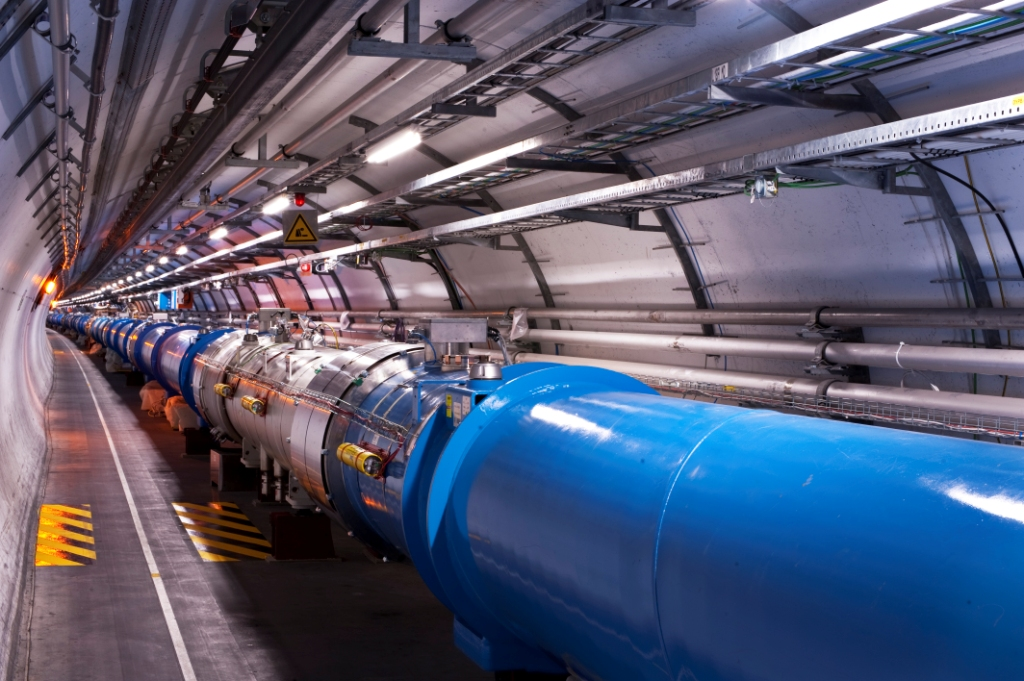
\includegraphics[width=200pt]{figures/lhc_cern_compressed.jpg}
    \end{figure}
  \end{frame}

  \begin{frame}{LWFA}
  Originally proposed by Toshiki Tajima and John Dawson in 1979
  \begin{figure}
    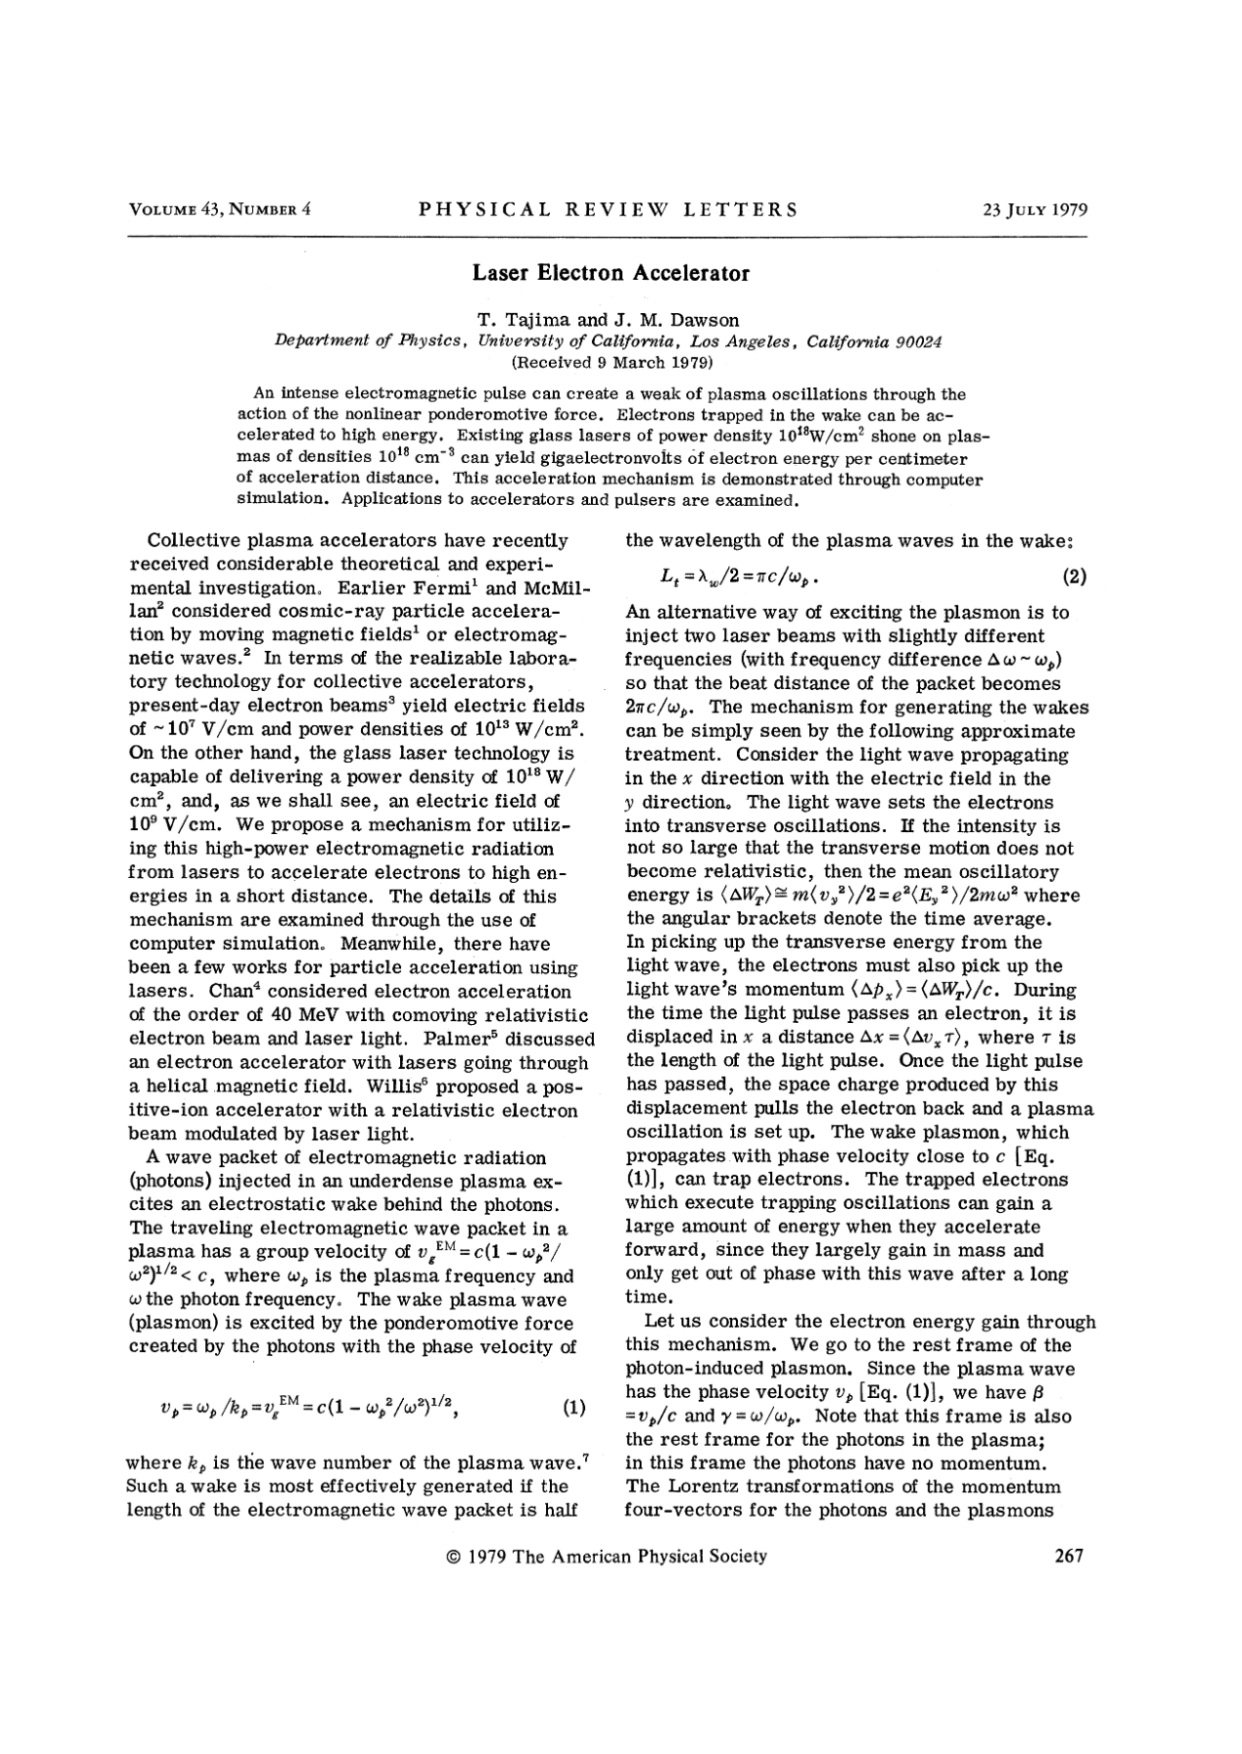
\includegraphics[height=0.7\textheight]{figures/PhysRevLett.43.267.pdf}
  \end{figure}
  \end{frame}
      
  \begin{frame}{LWFA}
  The idea: A plasma--based chraged particles accelerator.

  Electrical breakdown is part of the design.

  The power source is not microwave raidation, but either a laser beam or a charged partice beam.
  \begin{figure}
    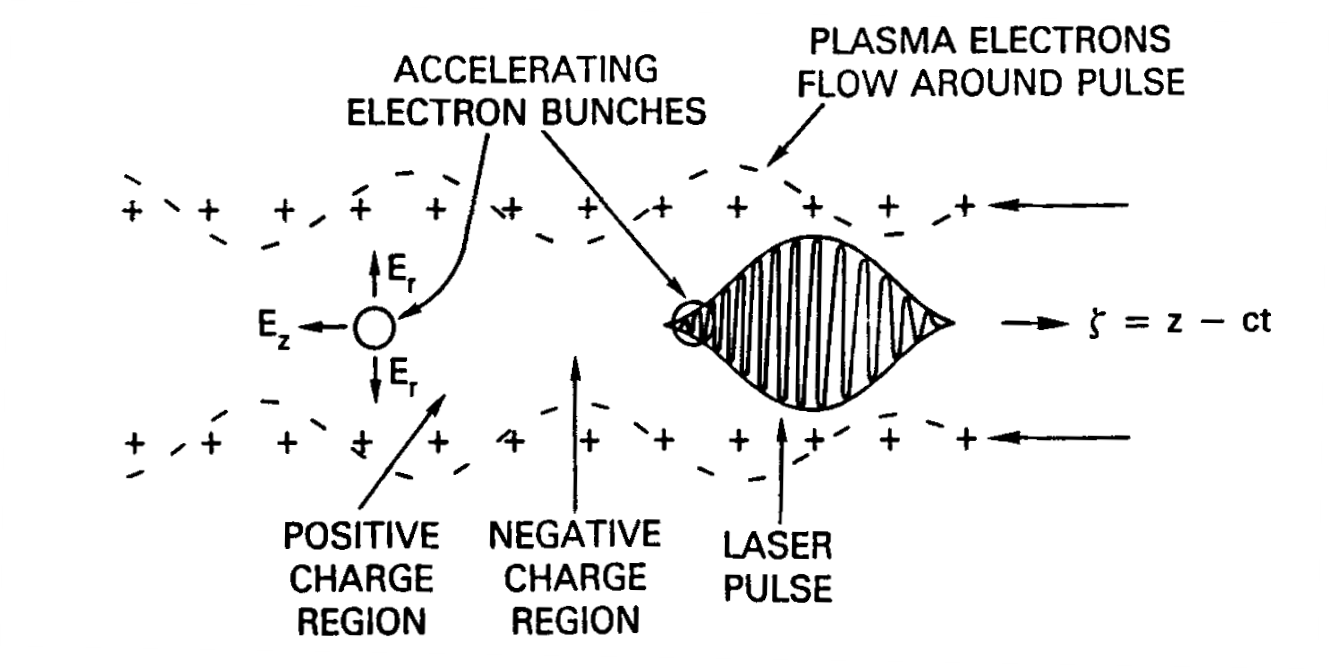
\includegraphics[width=300pt]{figures/lwfa-schematic.PNG}
  \end{figure}
  \end{frame}
  \begin{frame}{LWFA}{Limitations}
    \begin{columns}  
        \column{0.5\textwidth}<1>
    Defocusing of the laser radiation
      \begin{figure}
          \includegraphics[width=60pt]{figures/theory/fr1.png}
      \end{figure}
        \column{0.5\textwidth}<2>
      Electron dephasing length
      \begin{figure}
          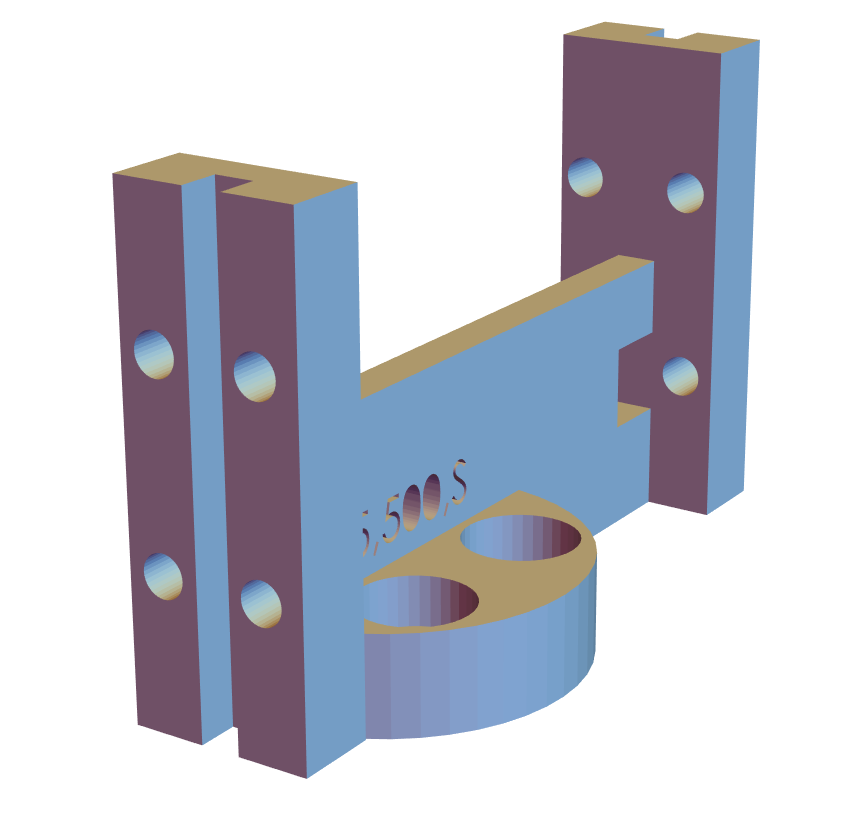
\includegraphics[width=0.3\textwidth]{figures/ablated.png}
      \end{figure}
    \end{columns}
  \end{frame}
  \subsection{Background to plasma}
  \begin{frame}{Measures}
  \begin{description}
      \item[Debye Length] $\lambda_D=\sqrt{\frac{\varepsilon_0 k_B T_e}{N_e e^2}}=\sqrt{\frac{k_B T}{m_e}}\frac{1}{\omega_p}$ 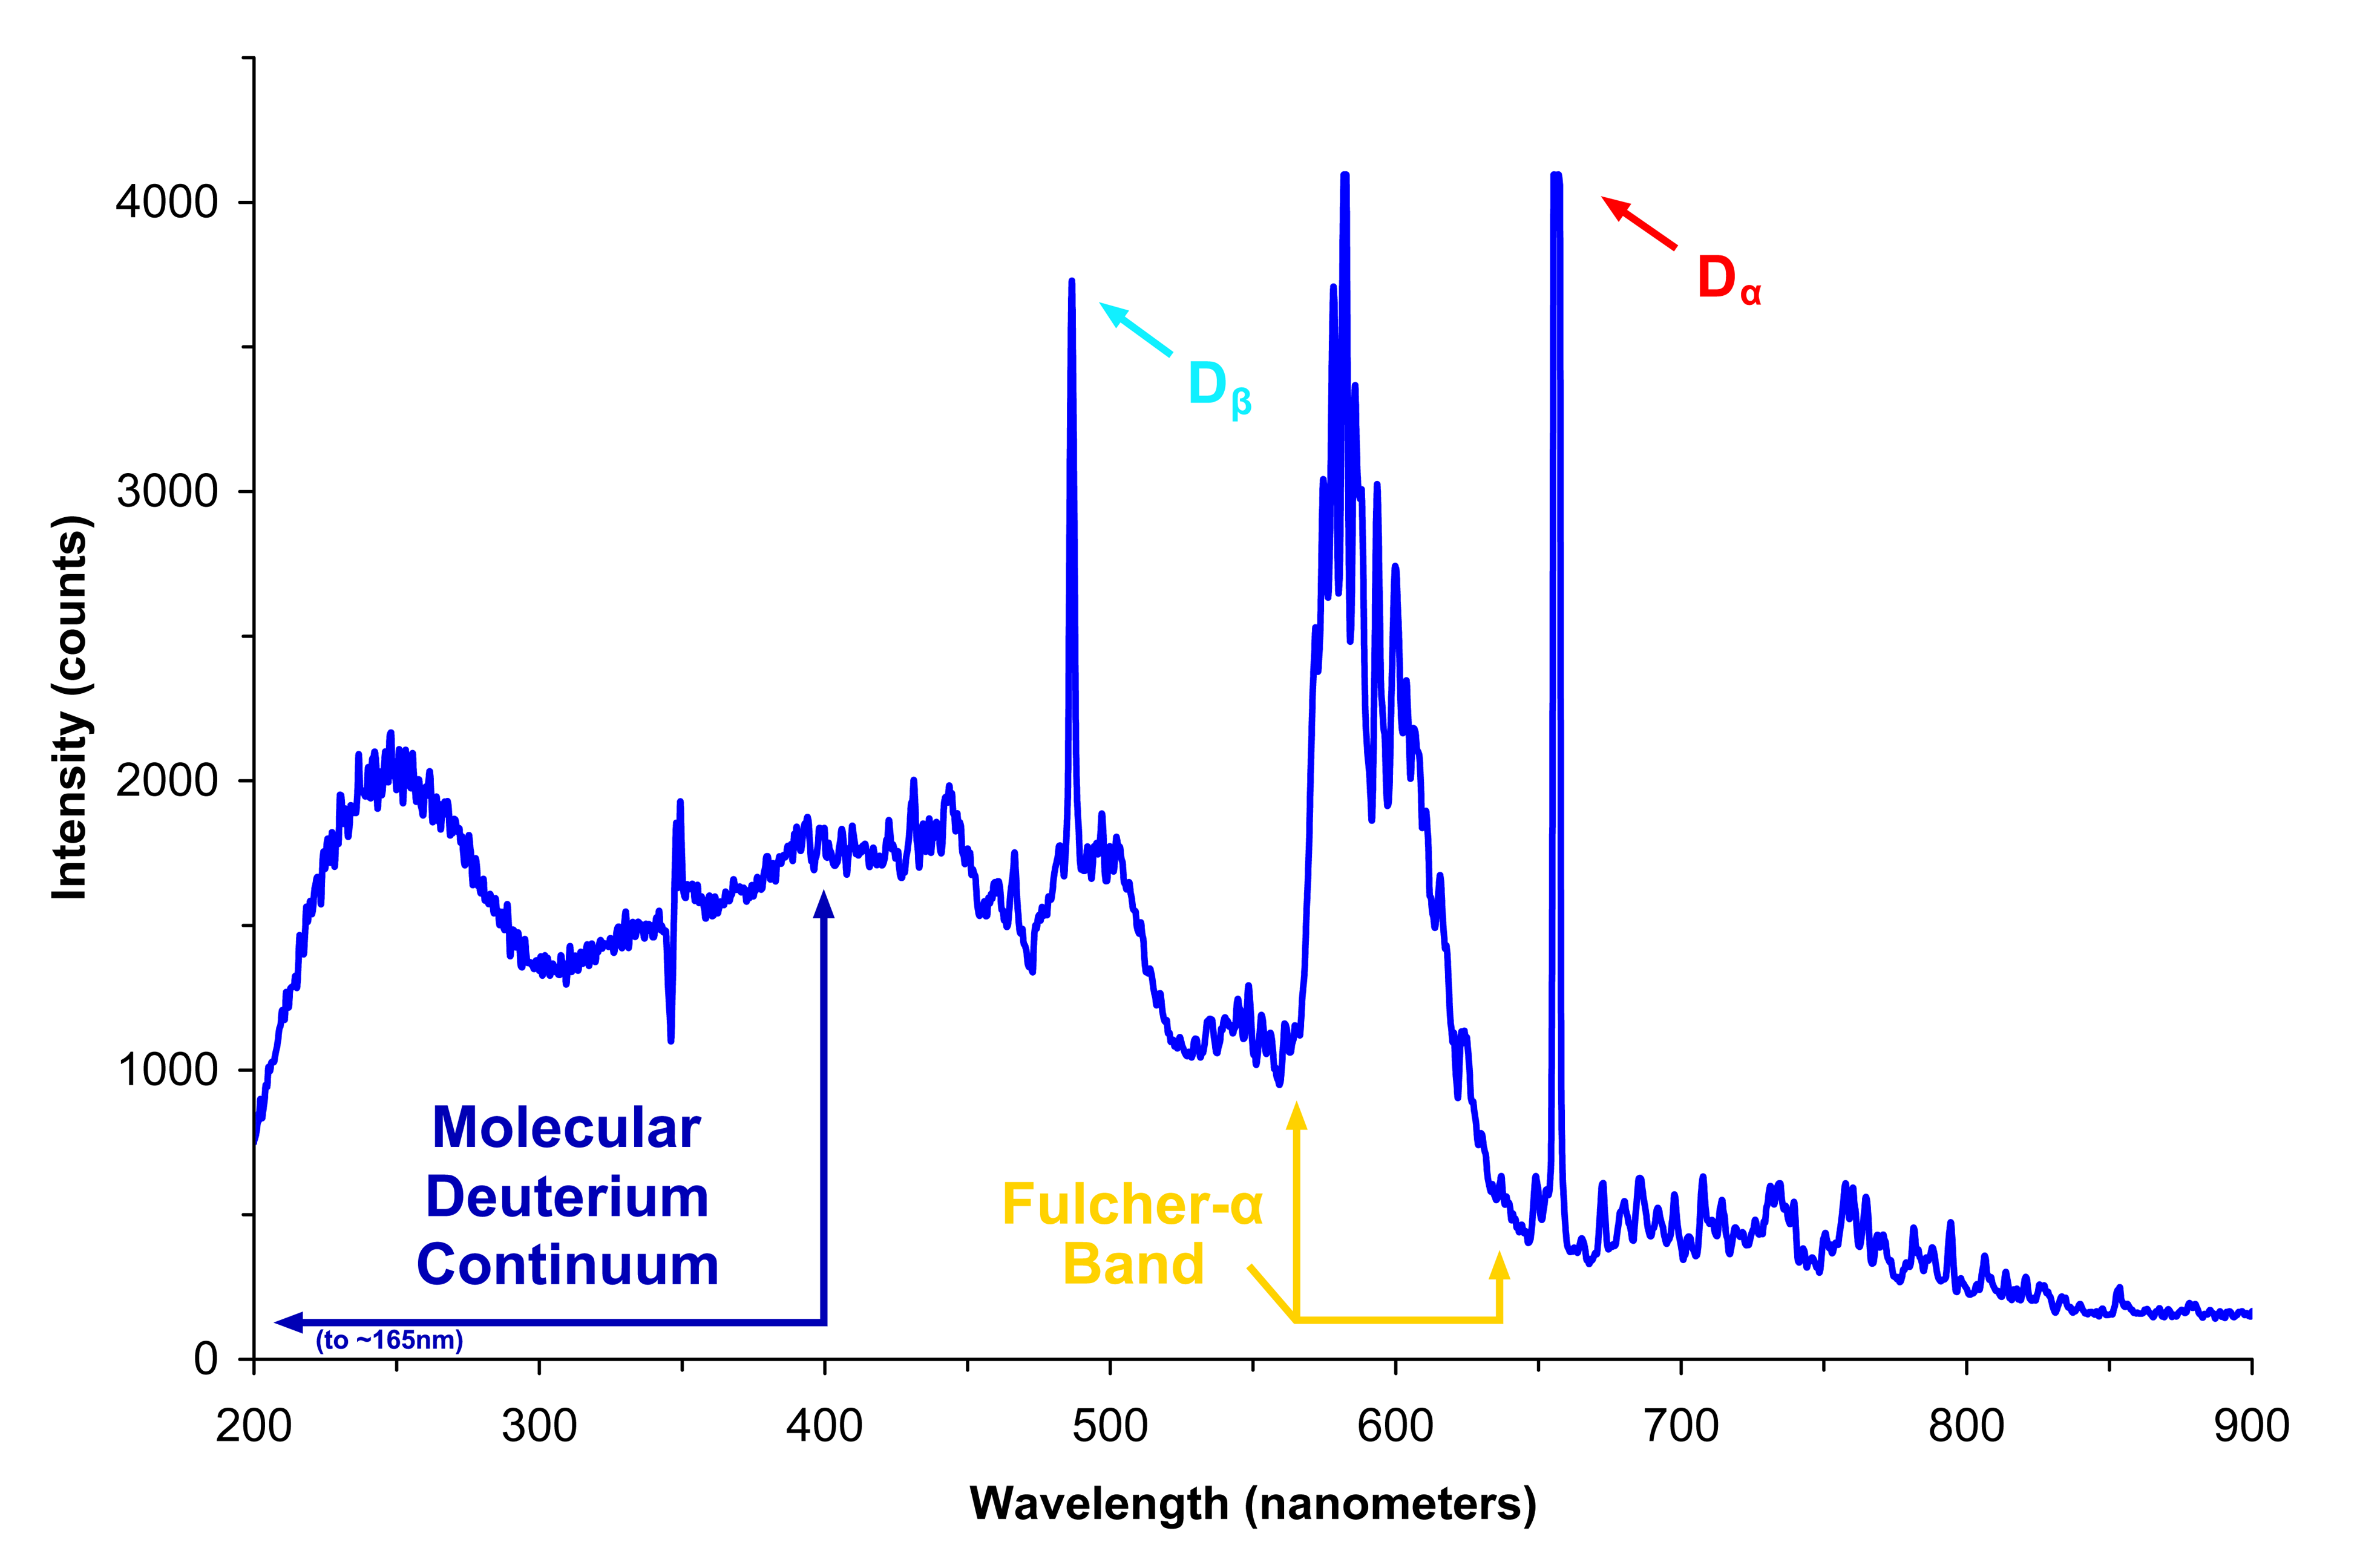
\includegraphics[width=.2\textwidth]{figures/Deuterium_lamp_1.png}
      \item[Plasma frequency] $ \omega_p=\sqrt{\frac{N_e e^2}{m_e \varepsilon_0}}\si[per-mode=fraction]{\radian\per\sec} $ 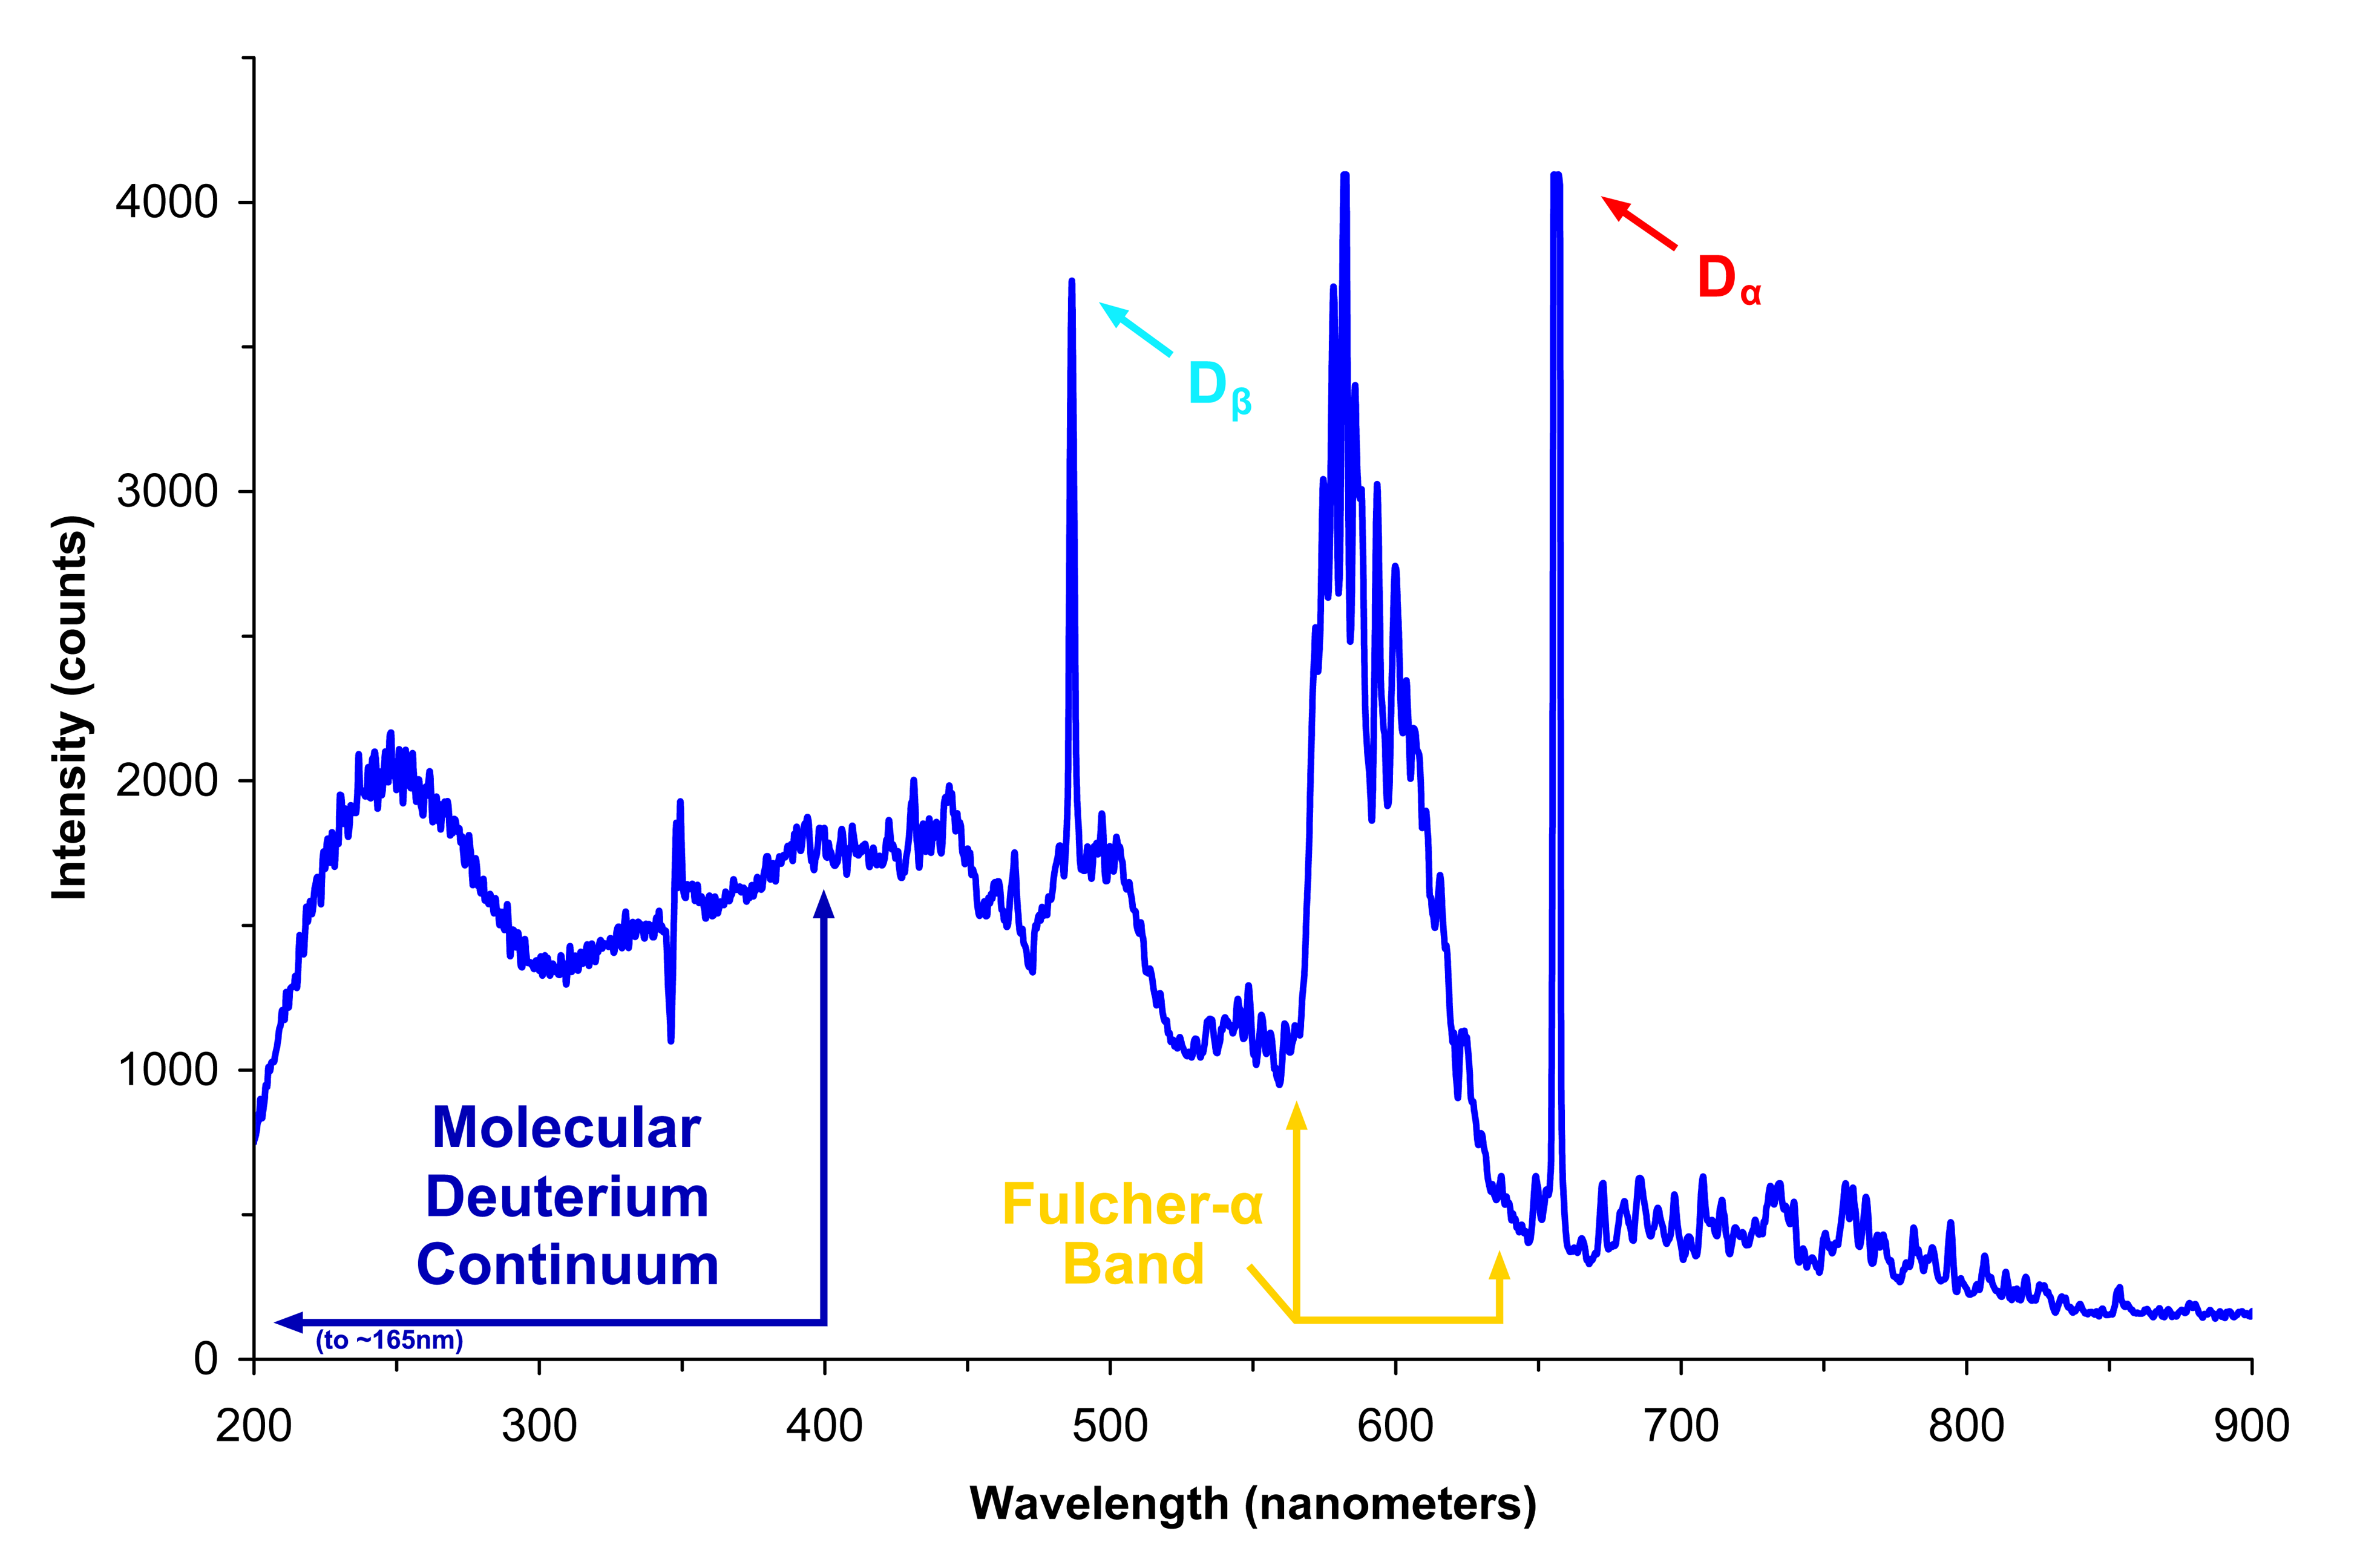
\includegraphics[width=.2\textwidth]{figures/Deuterium_lamp_1.png}
      \item[Plasma parameter] $ \Lambda=4\pi N_e \lambda_D ^3 $ 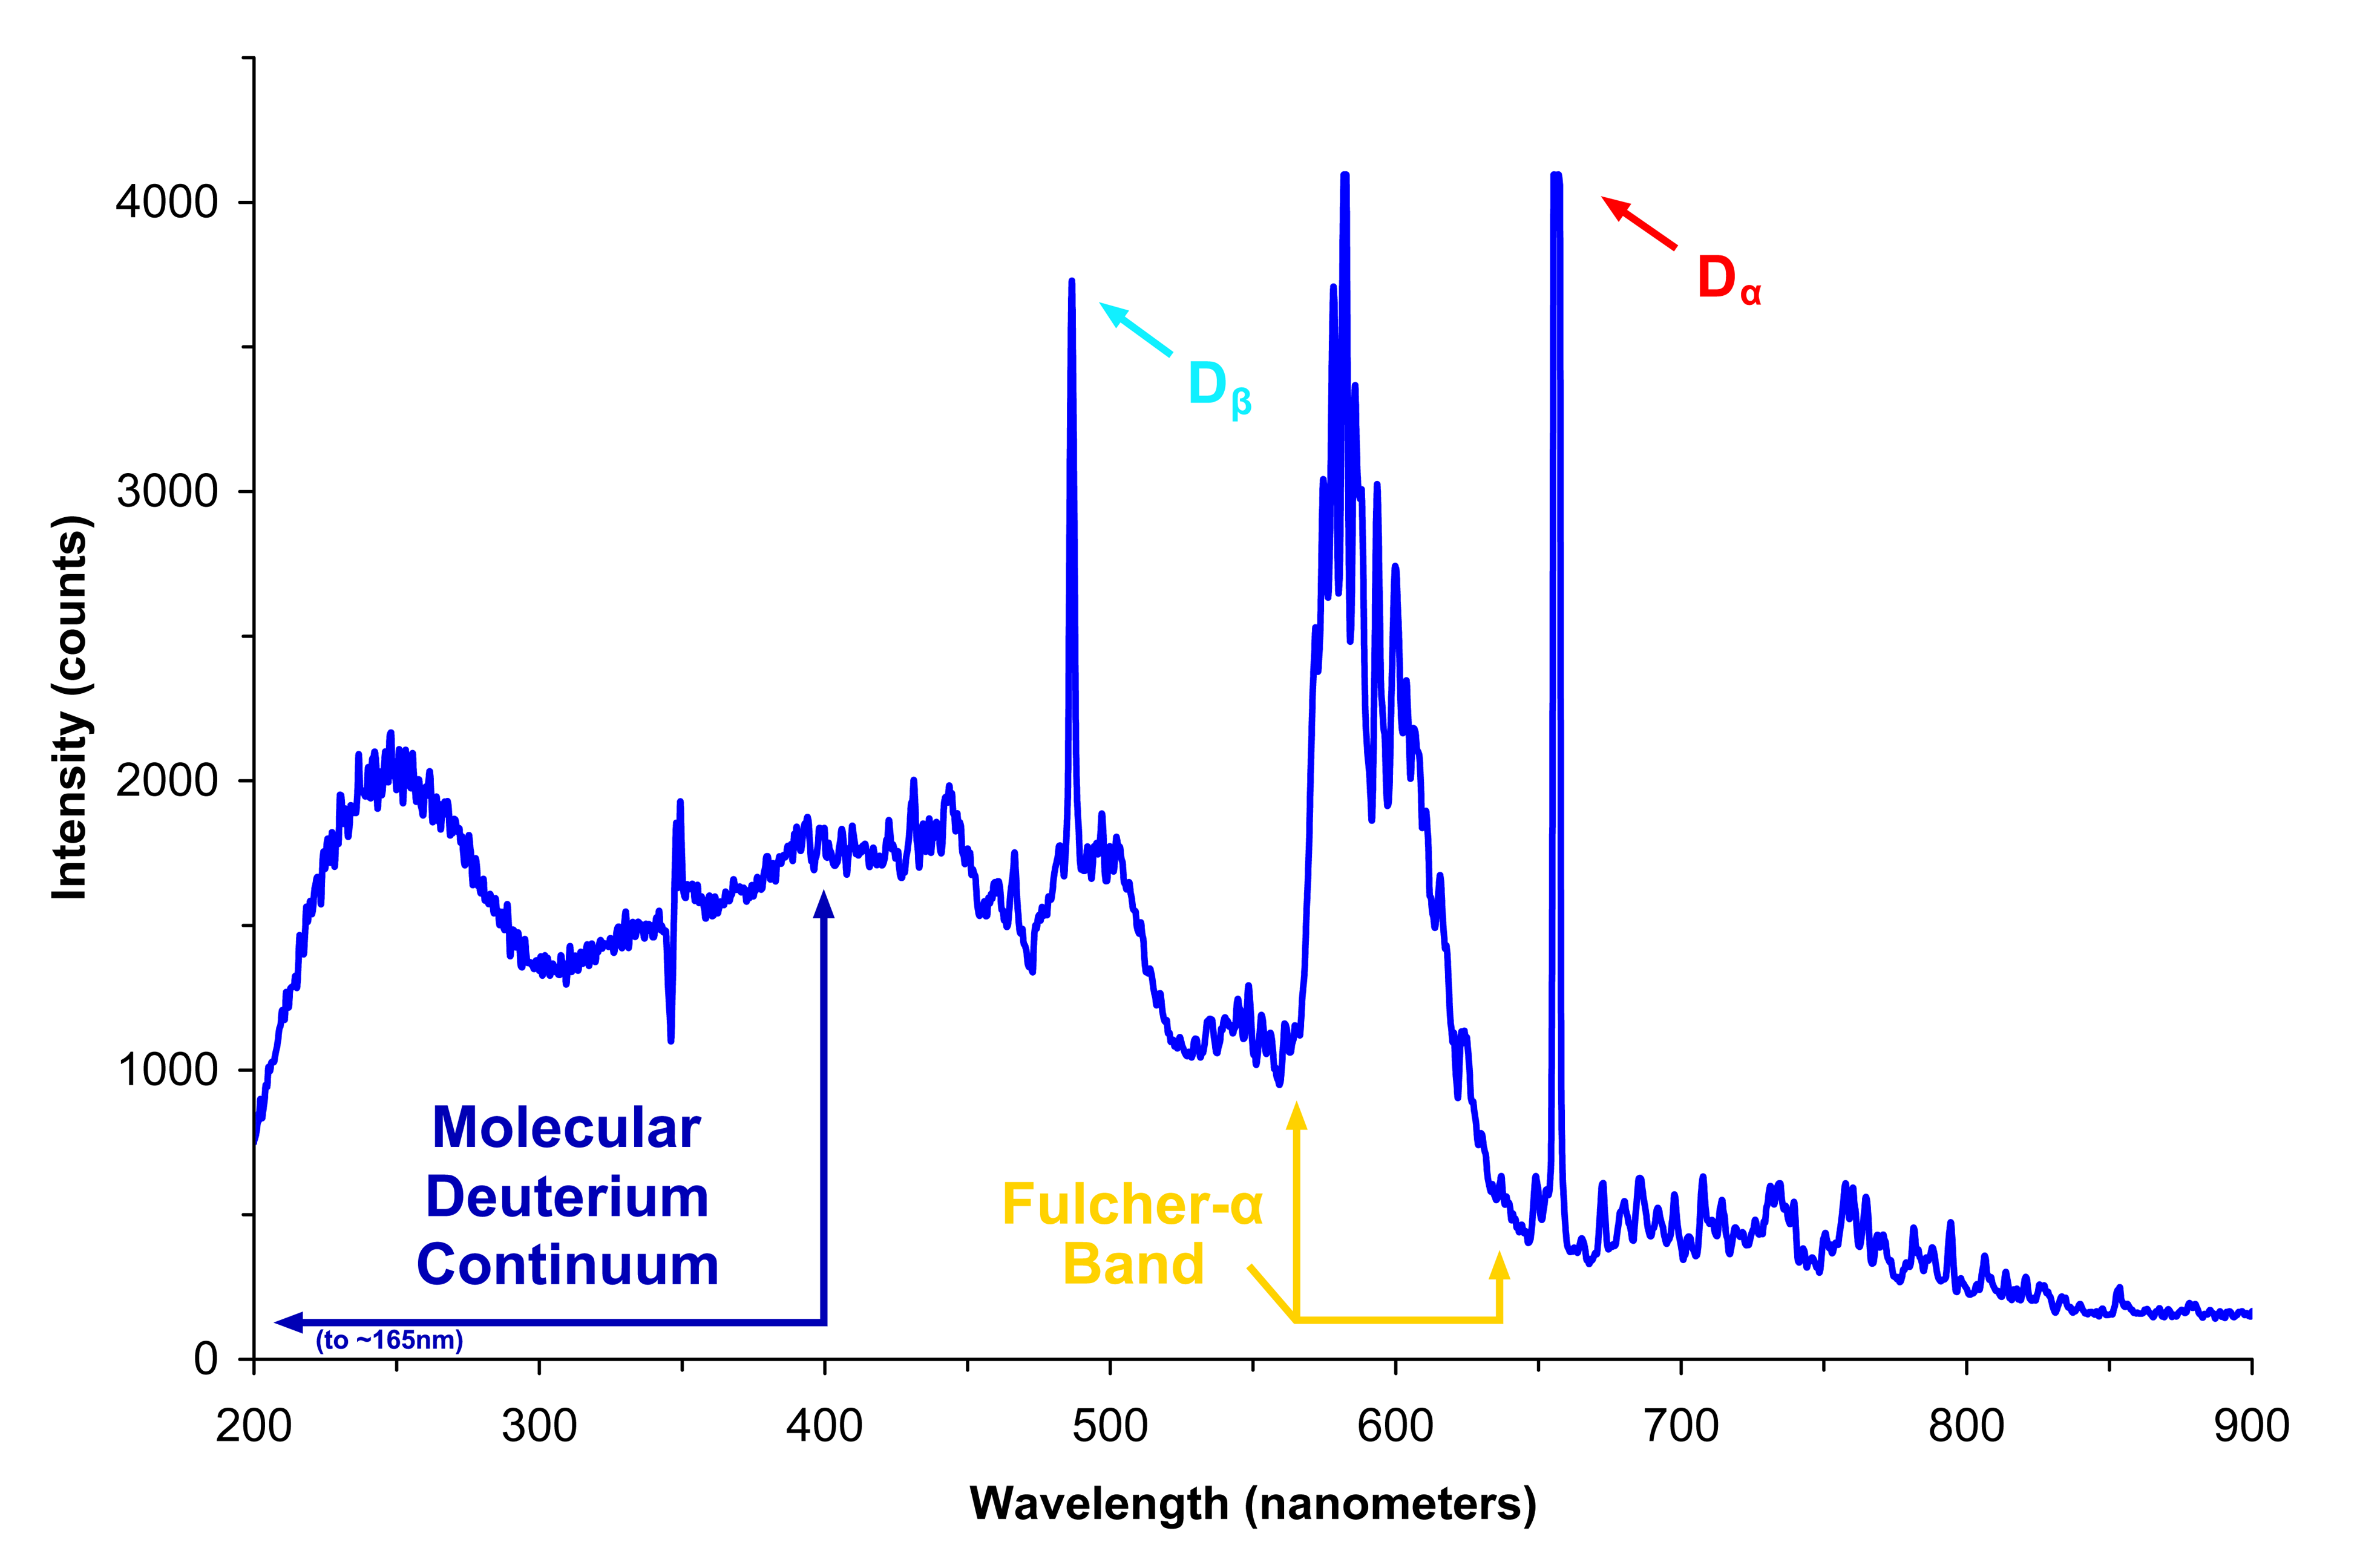
\includegraphics[width=.2\textwidth]{figures/Deuterium_lamp_1.png}
  \end{description}
  \end{frame}


\end{document}